\section{Bocetos}
Para realizar los bocetes se ha utilizado la herramienta Figma, que permite crear prototipos interactivos de forma sencilla y rápida. Los bocetos se han diseñado para reflejar la estructura y el flujo de navegación de la aplicación, así como para mostrar las 
principales funcionalidades y pantallas que se implementarán en el proyecto,
 para ver con mayor claridad se pueden usar el enlace :
 \newline 
 \url{https://www.figma.com/design/aNuYr9skZX7z6x5FqHQXfw/Trabajo-DGP?node-id=0-1&t=0Jn5VwT3RTUfXOOC-1}
\subsection{Bocetos Agenda}

Para ver de forma clara la estructura de la aplicación y cómo se conectan las distintas pantallas, en primer lugar, se incluye el esquema general de navegación y, a continuación, se explica en detalle cada uno de los flujos de la interfaz.

% ------------ IMAGEN: Esquema general de navegación ------------
\begin{figure}[H]
    \centering
     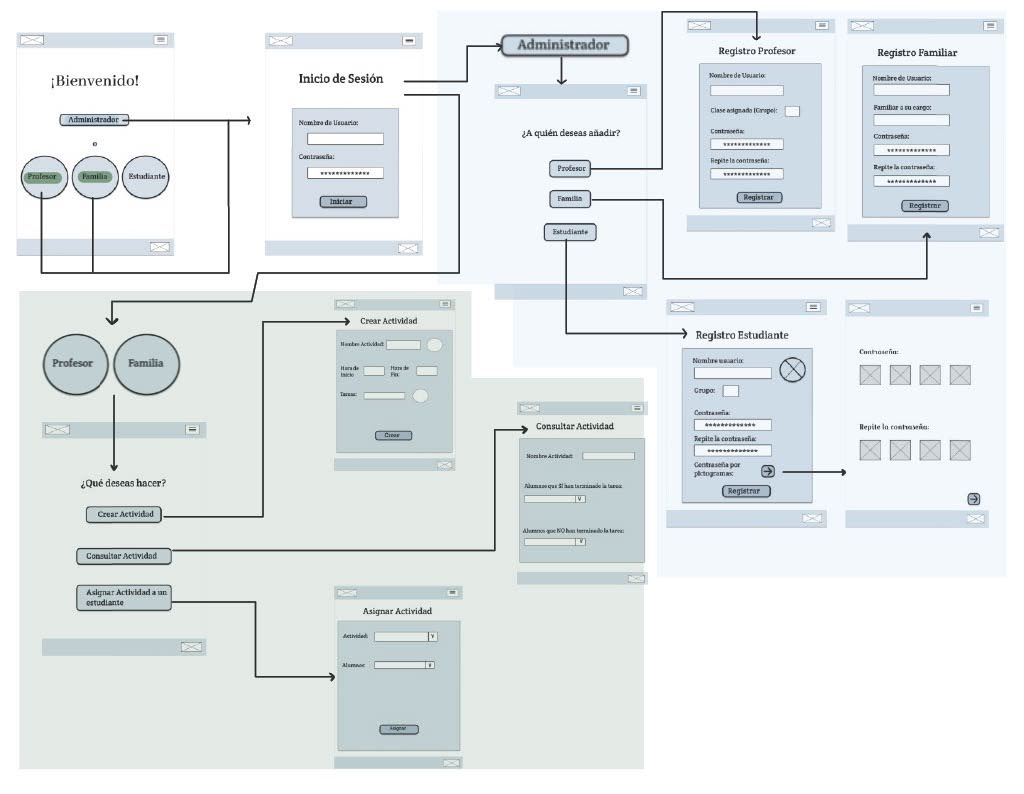
\includegraphics[width=1.2\textwidth]{img/primeraiteracion/esquema_general.png}
    \caption{Esquema general de navegación de la aplicación.}
    \label{fig:esquema_general}
\end{figure}

\begin{figure}[H]
    \centering
     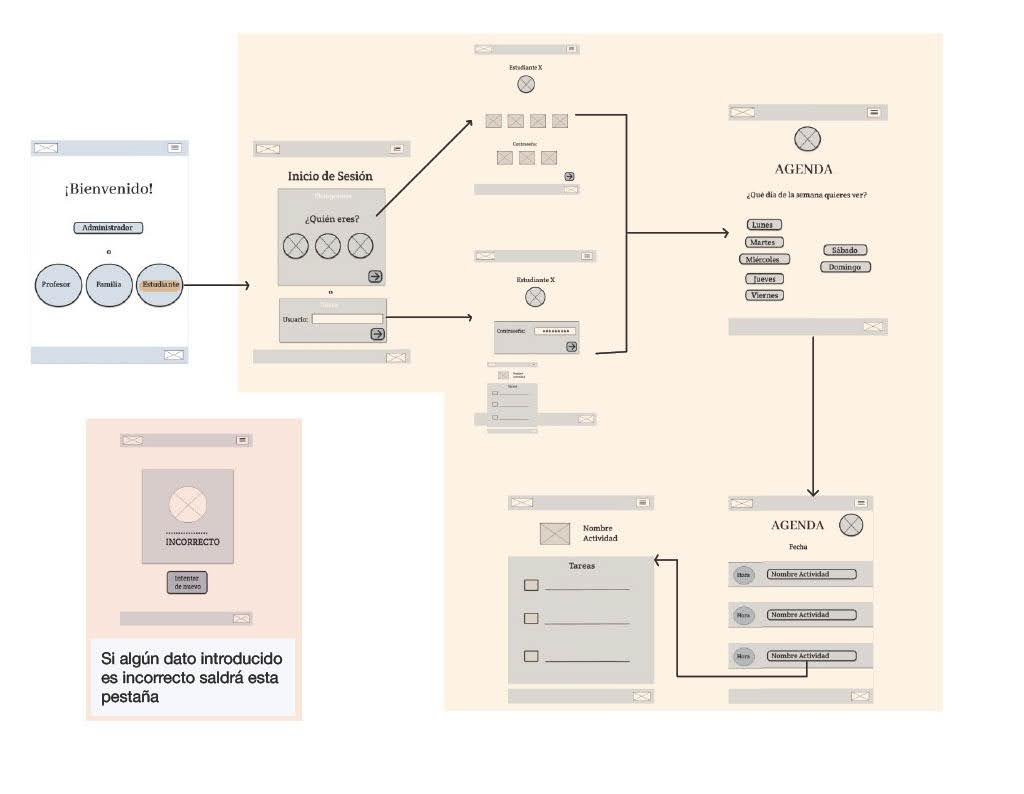
\includegraphics[width=1.2\textwidth]{img/primeraiteracion/esquema_general2.png}
    \caption{Esquema general de navegación de la aplicación.}
    \label{fig:esquema_general2}
\end{figure}
\newpage
En primer lugar, nos encontramos con una pantalla de bienvenida donde debemos elegir el perfil con el que deseamos acceder a la aplicación: Administrador, Profesor, Familia o Estudiante. Dependiendo de la opción escogida, el sistema redirige al usuario a su respectivo inicio de sesión o panel de control.

% ------------ IMAGEN: Pantalla de Bienvenida / Selección de Perfil ------------
\begin{figure}[H]
    \centering
    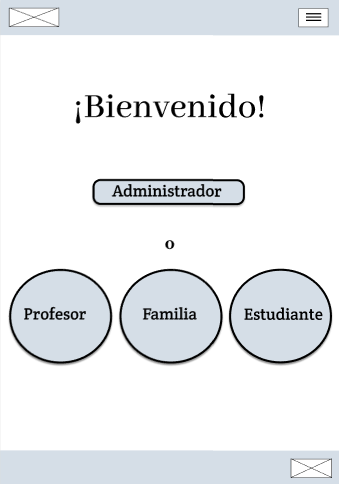
\includegraphics[width=0.6\textwidth]{img/primeraiteracion/pantalla_bienvenida.png}
    \caption{Pantalla de bienvenida y selección de perfil.}
    \label{fig:pantalla_bienvenida}
\end{figure}
\newpage
Si seleccionamos los perfiles de Administrador, Familiar o Profesor, la aplicación redirige a una interfaz de inicio de sesión unificada. En esta pantalla se solicita introducir el Nombre de Usuario y la Contraseña, con un botón para entrar a la aplicación.

% ------------ IMAGEN: Login Administrador, Profesor y Familia ------------
\begin{figure}[H]
    \centering
    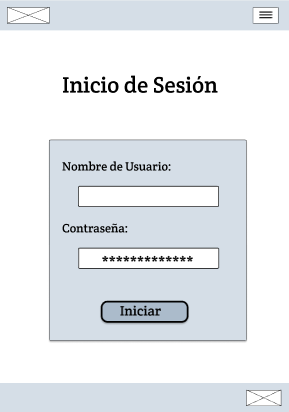
\includegraphics[width=0.8\textwidth]{img/primeraiteracion/login_unificado.png}
    \caption{Interfaz de inicio de sesión unificada para Administrador, Profesor y Familia.}
    \label{fig:login_unificado}
\end{figure}
\newpage
Por otro lado, si seleccionamos el inicio de sesión del estudiante, este ofrece dos alternativas adaptadas a las necesidades del usuario, ya que se puede identificar mediante pictogramas («¿Quién eres?») o introduciendo el nombre de usuario por texto. Dependiendo de la opción escogida, la aplicación redirige a una pantalla u otra para introducir la contraseña: si se entra por pictogramas, la clave se introduce también de forma visual mediante una secuencia de iconos y, si se accede por texto, se utiliza un campo de contraseña tradicional.

% ------------ IMAGEN: Login Estudiante (Texto vs Pictogramas) ------------
\begin{figure}[H]
    \centering
    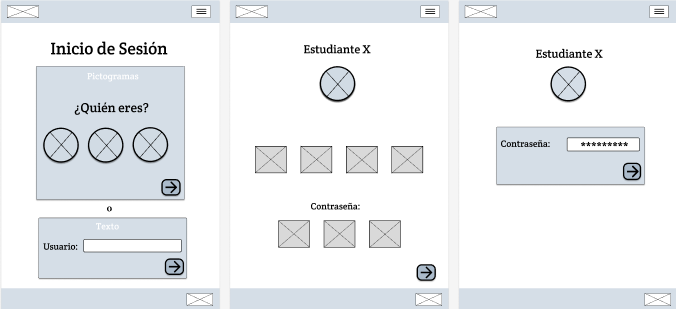
\includegraphics[width=0.6\textwidth]{img/primeraiteracion/login_estudiante.png}
    \caption{Opciones de inicio de sesión para el perfil de Estudiante.}
    \label{fig:login_estudiante}
\end{figure}
\newpage
Si iniciamos la sesión como Administrador, la interfaz muestra una pantalla con la pregunta «¿A quién deseas añadir?», permitiendo escoger entre tres opciones: Profesor, Familia o Estudiante. Dependiendo de la selección, el sistema redirige al usuario hacia el formulario de registro correspondiente para dar de alta al nuevo usuario en la plataforma.

\begin{figure}[H]
    \centering
    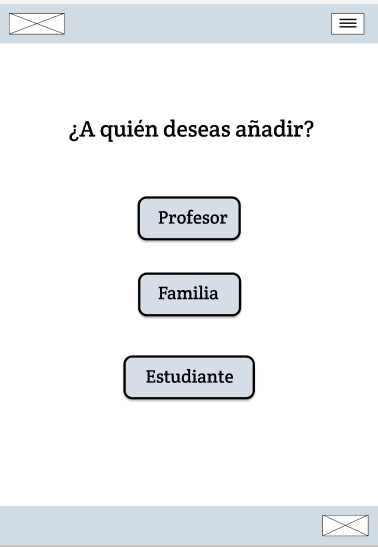
\includegraphics[width=0.6\textwidth]{img/primeraiteracion/interfaz_admin.png}
    \caption{Interfaz de administración para el perfil de Administrador.}
    \label{fig:interfaz_admin}
\end{figure}
\newpage
Si optamos por registrar un Profesor, la pantalla muestra un formulario donde se solicita el nombre de usuario, la clase asignada, la contraseña y su confirmación. De forma similar, si elegimos la opción de Familiar, el formulario solicita el nombre de usuario, el estudiante vinculado al familiar, la contraseña y su correspondiente repetición para validar el registro.

\begin{figure}[H]
    \centering
    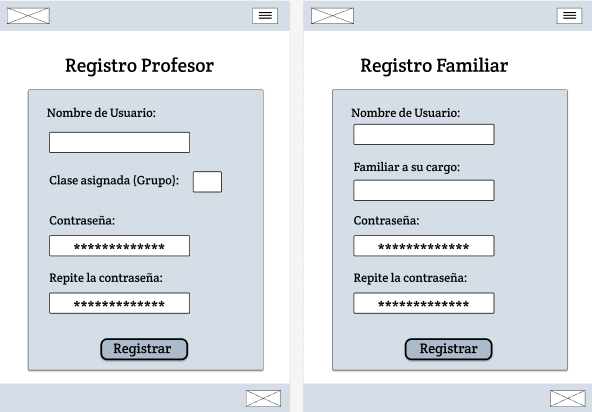
\includegraphics[width=0.8\textwidth]{img/primeraiteracion/registrar_profesor.png}
    \caption{Interfaz de registro de usuarios para los perfiles de Profesor y Familiar.}
    \label{fig:registrar_profesor}
\end{figure}
\newpage
Por otro lado, si elegimos la opción de Estudiante, accedemos a una pantalla de registro donde se solicita el nombre de usuario, el grupo y la contraseña mediante texto. No obstante, para aquellos estudiantes que se comunican o interactúan mejor de forma visual o que lo soliciten, la aplicación incluye la posibilidad de introducir y configurar la contraseña mediante pictogramas, donde de los cuatro pictogramas que se presentan, deberán seleccionar tres (pudiendo ser tres diferentes, tres iguales, dos iguales o la combinación que prefiera para su contraseña).

% ------------ IMAGEN: Formularios de Registro de Usuarios ------------
\begin{figure}[H]
    \centering
    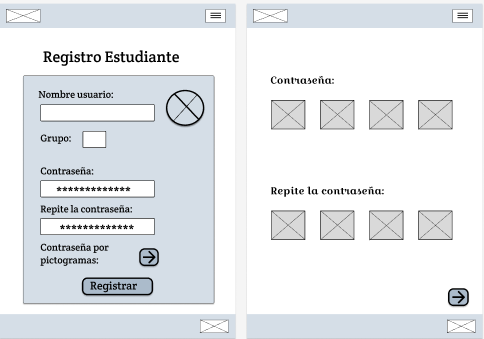
\includegraphics[width=0.8\textwidth]{img/primeraiteracion/registrar_estudiante.png}
    \caption{Interfaz de registro de usuarios para el perfil de Estudiante.}
    \label{fig:registrar_estudiante}
\end{figure}
\newpage
Si iniciamos sesión como Profesor o Familiar, la aplicación muestra una pantalla con la pregunta «¿Qué deseas hacer?». Desde aquí se puede elegir entre tres opciones principales mediante botones: «Crear Actividad», «Consultar Actividad» o «Asignar Actividad a un Estudiante».

% ------------ IMAGEN: Gestión de Actividades (Crear, Consultar y Asignar) ------------
\begin{figure}[H]
    \centering
    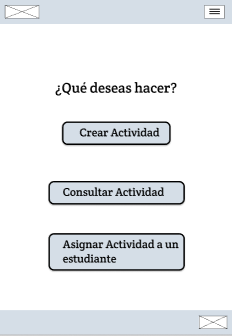
\includegraphics[width=0.6\textwidth]{img/primeraiteracion/gestion_actividades.png}
    \caption{Pantallas de gestión de actividades para Profesor y Familia.}
    \label{fig:gestion_actividades}
\end{figure}
\newpage
Si seleccionamos la opción de Crear Actividad, se despliega un formulario que permite configurar los detalles de la nueva actividad, donde se debe indicar el Nombre de la Actividad y el pictograma asociado, la Hora de Inicio y la Hora de Fin, así como un apartado para añadir las tareas vinculadas a la actividad y un botón de «Crear» para guardar los cambios.
\begin{figure}[H]
    \centering
    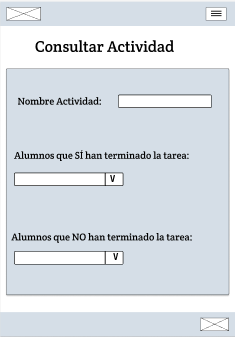
\includegraphics[width=0.6\textwidth]{img/primeraiteracion/crear_actividad.png}
    \caption{Pantallas de creación de actividades.}
    \label{fig:crear_actividad}
\end{figure}
\newpage
Por otro lado, si seleccionamos Consultar Actividad, accedemos a una pantalla de seguimiento que incluye el Nombre de la Actividad, las personas que la han completado y las personas que no. En el caso de los perfiles de Familiar, los listados desplegables de los alumnos que sí han terminado la tarea y de los alumnos que no han terminado la tarea se filtran de forma exclusiva para mostrar únicamente al alumno que tienen asociado a su cargo.
\begin{figure}[H]
    \centering
    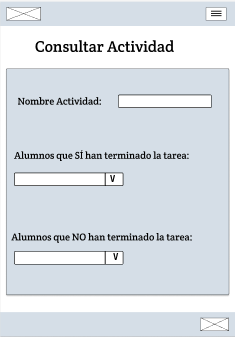
\includegraphics[width=0.6\textwidth]{img/primeraiteracion/consultar_actividad.png}
    \caption{Pantallas de consulta de actividades.}
    \label{fig:consultar_actividad}
\end{figure}
\newpage
Por último, si seleccionamos Asignar Actividad a un estudiante, tenemos dos campos desplegables: uno para seleccionar la Actividad y otro para elegir el Alumno o Alumnos al que se le va a asignar, finalizando con un botón de «Asignar». De igual forma que en «Consultar Actividad», si el usuario que realiza la acción es un Familiar, el desplegable de alumnos se restringe de forma que solo muestra al alumno que tiene a su cargo.
\begin{figure}[H]
    \centering
    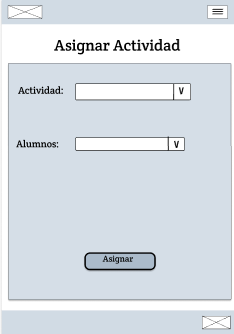
\includegraphics[width=0.6\textwidth]{img/primeraiteracion/asignar_actividad.png}
    \caption{Pantallas de asignación de actividades.}
    \label{fig:asignar_actividad}
\end{figure}
\newpage
Si iniciamos sesión como estudiante, se muestra la pantalla principal de su Agenda, donde se encuentra su imagen de usuario en la parte superior. Bajo el título, se plantea la pregunta «¿Qué día de la semana quieres ver?» y se presentan botones para seleccionar cada uno de los días.
\begin{figure}[H]
    \centering
    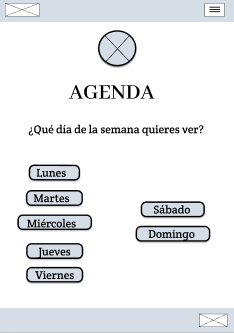
\includegraphics[width=0.6\textwidth]{img/primeraiteracion/panel_agenda.png}
    \caption{Pantalla principal de la Agenda del Estudiante.}
    \label{fig:panel_agenda}
\end{figure}
\newpage
Al pulsar sobre cualquiera de los días de la semana, la aplicación muestra la vista detallada de la Agenda para esa fecha concreta. En esta pantalla se despliega un listado con las actividades programadas, mostrando para cada una de ellas un círculo con la Hora de realización y un cuadro con el Nombre de la Actividad (que podrán ponerse en formato texto o con pictogramas).
\begin{figure}[H]
    \centering
    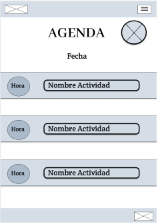
\includegraphics[width=0.6\textwidth]{img/primeraiteracion/vista_detalle_agenda.png}
    \caption{Pantalla principal, diaria y de detalle de tareas para el perfil Estudiante.}
    \label{fig:vista_detalle_agenda}
\end{figure}
\newpage
Al pulsar sobre una actividad específica, se accede a su pantalla de detalle. En la cabecera se muestra el Nombre de la Actividad acompañada de su pictograma asociado. Debajo, en la sección de Tareas, se despliega el listado donde cada elemento puede presentarse mediante texto o pictogramas dependiendo de la configuración del estudiante, incluyendo una casilla cuadrada a la izquierda diseñada para que el alumno pueda marcar la tarea como completada.

% ------------ IMAGEN: Vistas de la Agenda de Estudiante ------------
\begin{figure}[H]
    \centering
    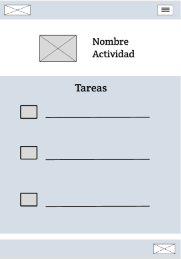
\includegraphics[width=0.6\textwidth]{img/primeraiteracion/detalle_actividad.png}
    \caption{Vista de detalle de una actividad en la Agenda del Estudiante.}
    \label{fig:detalle_actividad}
\end{figure}
\newpage
Para finalizar, la aplicación cuenta con una pantalla de error. En caso de que se introduzca un campo incorrecto en cualquiera de los formularios o procesos (como la contraseña o el nombre de usuario), el sistema redirige a esta interfaz, donde se muestra un icono superior, el texto correspondiente indicando qué campo ha sido incorrecto y un botón de «Intentar de nuevo» para volver a la pantalla anterior.

% ------------ IMAGEN: Pantalla de Error ------------
\begin{figure}[H]
    \centering
    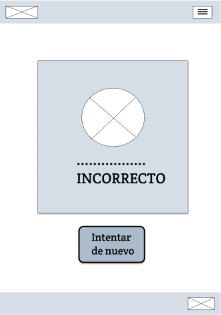
\includegraphics[width=0.6\textwidth]{img/primeraiteracion/pantalla_error.png}
    \caption{Pantalla de error en el sistema.}
    \label{fig:pantalla_error}
\end{figure}

\subsection{Bocetos Base de Datos}
\begin{figure}[H]
    \centering
    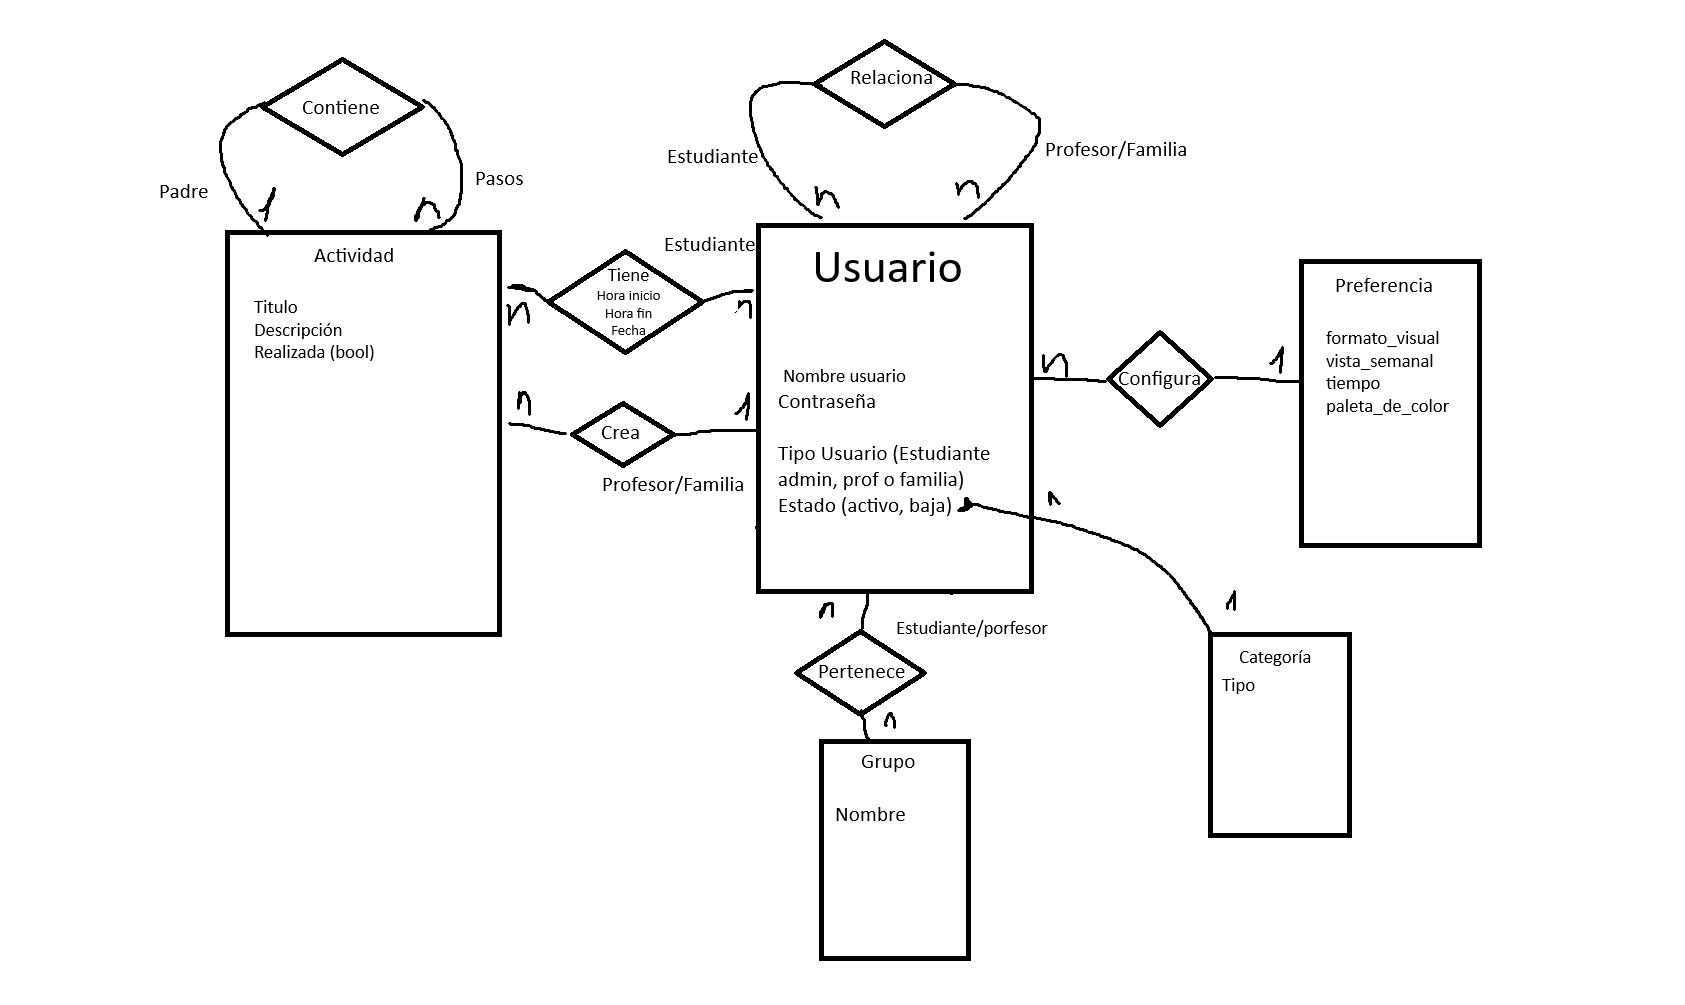
\includegraphics[width=1.2\textwidth]{img/primeraiteracion/bd_boceto.png}
    \caption{Boceto de la Base de Datos.}
    \label{fig:bd_boceto}
\end{figure}

